% =========================================================================
% ARCHIVO AUXILIAR - TEMA 3: TEORÍA DE PEANO
% (Este archivo no está incluido en Theory.tex ni en la compilación principal.
%  Creado para consulta y copiado progresivo hacia el archivo de trabajo).
% =========================================================================

\section{Teora de Peano}

\subsection{El problema de Cauchy bajo continuidad y el fenmeno de no unicidad}

Hasta ahora hemos estudiado problemas de Cauchy bajo hiptesis Lipschitzianas, donde el Teorema de Picard-Lindelf garantizaba no slo la existencia local, sino la unicidad rigurosa y la prolongabilidad maximal de las soluciones. Sin embargo, en mltiples modelos fsicos y biolgicos la velocidad de variacin no satisface una condicin Lipschitziana uniforme.

Consideremos un problema de Cauchy general:
\[
    \begin{cases}
        u' = f(t, u) \\
        u(t_0) = u_0 \in \Omega \subset \mathbb{R}^N
    \end{cases}
\]
donde $J \subset \mathbb{R}$ es un intervalo abierto que contiene a $t_0$, $\Omega \subset \mathbb{R}^N$ es un abierto, y el campo $f: J \times \Omega \to \mathbb{R}^N$ se asume \textbf{nicamente continuo}:
\[
    f \in \mathcal{C}(J \times \Omega; \, \mathbb{R}^N)
\]
Bajo estas condiciones mnimas, el panorama analtico cambia drsticamente: \textbf{en general, no existe unicidad de soluciones}.

\ejemplo{
    \textbf{Prdida de unicidad con campo no Lipschitziano:}

    Consideremos el problema autnomo escalar:
    \[
        \begin{cases}
            u' = \sqrt{|u|} \\
            u(0) = 0
        \end{cases}
    \]
    La funcin $f(u) = \sqrt{|u|}$ es continua en todo $\mathbb{R}$, pero su derivada:
    \[
        f'(u) = \frac{1}{2\sqrt{u}} \xrightarrow{u \to 0^+} +\infty
    \]
    no est acotada en ningn entorno del origen, por lo que $f$ no es Lipschitziana en $u = 0$.

    Este problema admite infinitas soluciones distintas. En primer lugar, la solucin idnticamente nula:
    \[
        u_0(t) = 0 \qquad \forall t \in \mathbb{R}
    \]
    Adems, para cualquier constante $c \geq 0$, la funcin:
    \[
        \varphi_c(t) = \begin{cases}
            0 & \text{si } t \leq c \\
            \dfrac{(t - c)^2}{4} & \text{si } t > c
        \end{cases}
    \]
    es de clase $\mathcal{C}^1(\mathbb{R})$ y satisface $\varphi_c(0) = 0$ y $\varphi_c'(t) = \sqrt{|\varphi_c(t)|}$ para todo $t \in \mathbb{R}$. Obtenemos as una familia no numerable de soluciones que se bifurcan a partir del punto de equilibrio.

    \begin{center}
    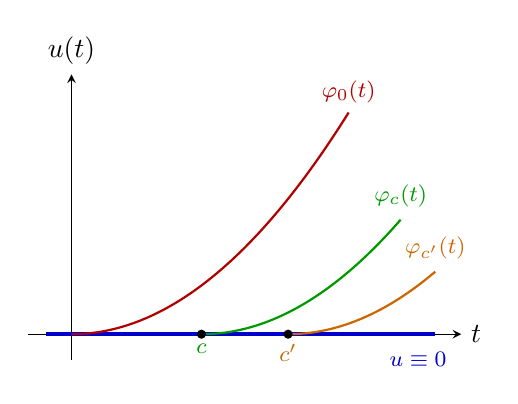
\begin{tikzpicture}[>=stealth, scale=1.1]
        % Ejes
        \draw[->] (-0.5,0) -- (4.5,0) node[right] {$t$};
        \draw[->] (0,-0.3) -- (0,3.0) node[above] {$u(t)$};
        
        % Solución idénticamente nula
        \draw[ultra thick, blue!80!black] (-0.3,0) -- (4.2,0);
        \node[below, blue!80!black, font=\footnotesize] at (4.0,-0.1) {$u \equiv 0$};
        
        % Solución para c = 0
        \draw[thick, red!70!black, domain=0:3.2, samples=60]
            plot (\x, {0.25*\x*\x});
        \node[above, red!70!black, font=\footnotesize] at (3.2,2.56) {$\varphi_0(t)$};
        
        % Solución para c = 1.5
        \draw[thick, green!60!black, domain=1.5:3.8, samples=60]
            plot (\x, {0.25*(\x - 1.5)*(\x - 1.5)});
        \node[above, green!60!black, font=\footnotesize] at (3.8,1.35) {$\varphi_c(t)$};
        \fill (1.5,0) circle (1.5pt);
        \node[below, green!60!black, font=\footnotesize] at (1.5,0) {$c$};
        
        % Solución para c = 2.5
        \draw[thick, orange!80!black, domain=2.5:4.2, samples=60]
            plot (\x, {0.25*(\x - 2.5)*(\x - 2.5)});
        \node[above, orange!80!black, font=\footnotesize] at (4.2,0.75) {$\varphi_{c'}(t)$};
        \fill (2.5,0) circle (1.5pt);
        \node[below, orange!80!black, font=\footnotesize] at (2.5,0) {$c'$};
    \end{tikzpicture}
    \end{center}
}

Para garantizar la existencia de al menos una solucin bajo la sola hiptesis de continuidad, el principio de contraccin de Banach resulta inoperante. La herramienta fundamental de Anlisis Funcional que sustituye a las contracciones es el \textbf{Teorema de Ascoli-Arzel} (desarrollado entre 1883 y 1895).

\subsection{Compacidad en espacios de Banach}

Sea $E$ un espacio de Banach (un espacio vectorial normado y completo sobre $\mathbb{R}$ con norma $\|\cdot\|_E$).

\begin{definicin}[Conjunto relativamente compacto]
    Un subconjunto $X \subseteq E$ se dice \textbf{relativamente compacto} si su clausura $\overline{X}$ es un conjunto compacto en $(E, \|\cdot\|_E)$. En tal caso, $X$ es necesariamente acotado.
\end{definicin}

La compacidad se caracteriza secuncialmente en espacios normados mediante el siguiente resultado clsico:

\begin{teorema}[Caracterizacin de relativa compacidad]
    Sea $E$ un espacio de Banach y $X \subseteq E$. Las siguientes afirmaciones son equivalentes:
    \begin{itemize}
        \item $X$ es relativamente compacto en $E$.
        \item De toda sucesin infinita $\{x_n\}_{n \geq 1} \subset X$ se puede extraer una subsucesin $\{x_{n_m}\}_{m \geq 1}$ convergente en $E$ a un punto del cierre $\overline{X}$.
    \end{itemize}
\end{teorema}

\textbf{El caso de dimensin finita ($E = \mathbb{R}^N$):}

En espacios eucldeos de dimensin finita, el Teorema de Bolzano-Weierstrass establece que todo conjunto acotado posee subsucesiones convergentes:
\[
    X \subset \mathbb{R}^N \text{ relativamente compacto} \iff \overline{X} \text{ es cerrado y acotado} \iff X \text{ es acotado}
\]
Por consiguiente, en $\mathbb{R}^N$ los conjuntos relativamente compactos son exactamente los conjuntos acotados.

\medskip

\textbf{El problema en dimensin infinita:}

Consideremos un subconjunto compacto no vaco $K \subset \mathbb{R}^M$ y el espacio vectorial de las funciones continuas $\mathcal{C}(K; \, \mathbb{R}^N)$ dotado de la norma del supremo:
\[
    \|u\|_\infty = \max_{x \in K} \|u(x)\|
\]
El espacio $(\mathcal{C}(K; \, \mathbb{R}^N), \, \|\cdot\|_\infty)$ es un espacio de Banach de dimensin infinita. Surge de manera natural la cuestin: \textit{¿cules son los subconjuntos $\mathcal{F} \subset \mathcal{C}(K; \, \mathbb{R}^N)$ relativamente compactos? ¿Basta que una familia sea acotada?}

La respuesta es rotundamente \textbf{NO}: en dimensin infinita existen familias acotadas que no admiten ninguna subsucesin convergente.

\subsubsection{Contraejemplo: insuficiencia de la acotacin uniforme}

Para ilustrar este fenmeno, consideremos en el espacio $\mathcal{C}([0, 1]; \, \mathbb{R})$ la sucesin de funciones potenciales:
\[
    f_n: [0, 1] \to \mathbb{R}, \qquad f_n(t) = t^n \quad (n \geq 1)
\]
Cada funcin $f_n$ es continua en $[0, 1]$, y la familia $\mathcal{F} = \{f_n\}_{n \geq 1}$ est acotada en norma del supremo:
\[
    |f_n(t)| = |t^n| \leq 1 \implies \|f_n\|_{\infty, [0, 1]} = 1 \qquad \forall n \geq 1
\]
Analicemos el lmite puntual de $f_n$ cuando $n \to \infty$:
\[
    f(t) = \lim_{n \to \infty} t^n = \begin{cases}
        0 & \text{si } t \in [0, 1) \\
        1 & \text{si } t = 1
    \end{cases}
\]
La funcin lmite $f(t)$ presenta una discontinuidad inevitable de salto en $t = 1$.

\begin{proposicin}[No compacidad de la familia de potencias]
    La familia $\mathcal{F} = \{f_n\}_{n \geq 1} = \{t^n\}_{n \geq 1}$ no es relativamente compacta en $\mathcal{C}([0, 1]; \, \mathbb{R})$.
\end{proposicin}

\begin{proof}
    Razonemos por reduccin al absurdo. Supongamos que $\mathcal{F}$ fuera relativamente compacta en $\mathcal{C}([0, 1]; \, \mathbb{R})$. Entonces existira una subsucesin $\{f_{n_m}\}_{m \geq 1} \subset \mathcal{F}$ convergente en la norma $\|\cdot\|_\infty$ a alguna funcin $g \in \mathcal{C}([0, 1]; \, \mathbb{R})$:
    \[
        \lim_{m \to \infty} \|f_{n_m} - g\|_\infty = 0
    \]
    La convergencia uniforme implica que $f_{n_m}(t)$ converge puntualmente a $g(t)$ para todo $t \in [0, 1]$:
    \[
        g(t) = \lim_{m \to \infty} f_{n_m}(t) \qquad \forall t \in [0, 1]
    \]
    Por otra parte, como cualquier subsucesin de una sucesin convergente comparte el mismo lmite puntual, se tiene forzosamente que $g(t) = f(t)$ para todo $t \in [0, 1]$, siendo $f$ la funcin discontinua obtenida anteriormente:
    \[
        g(t) = \begin{cases}
            0 & \text{si } t \in [0, 1) \\
            1 & \text{si } t = 1
        \end{cases}
    \]
    Esto entra en contradiccin directa con el hecho de que $g \in \mathcal{C}([0, 1]; \, \mathbb{R})$. Concluimos que de la sucesin acotada $\{f_n\}$ no puede extraerse ninguna subsucesin convergente en $\mathcal{C}([0, 1]; \, \mathbb{R})$, luego $\mathcal{F}$ no es relativamente compacta.
\end{proof}

\begin{center}
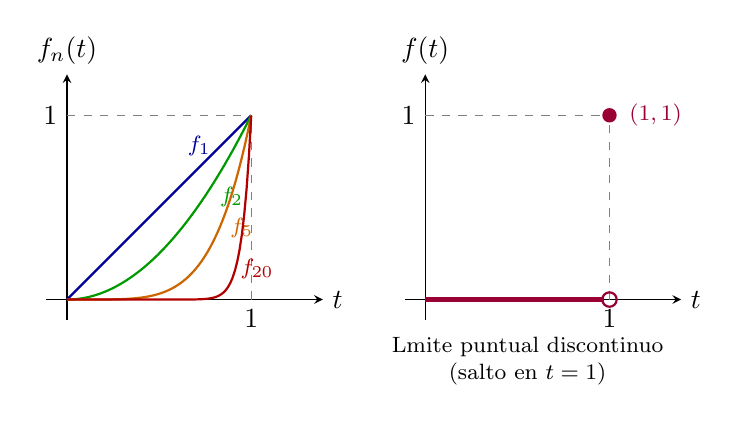
\begin{tikzpicture}[>=stealth, scale=1.3]
    % Ejes
    \draw[->] (-0.2,0) -- (2.5,0) node[right] {$t$};
    \draw[->] (0,-0.2) -- (0,2.2) node[above] {$f_n(t)$};
    
    % Cuadrado unitario
    \draw[dashed, gray] (1.8,0) node[below, black] {$1$} -- (1.8,1.8);
    \draw[dashed, gray] (0,1.8) node[left, black] {$1$} -- (1.8,1.8);
    
    % Curvas t^n
    \draw[thick, blue!60!black, domain=0:1.8, samples=50]
        plot (\x, {\x});
    \node[left, blue!60!black, font=\footnotesize] at (1.5,1.5) {$f_1$};
    
    \draw[thick, green!60!black, domain=0:1.8, samples=50]
        plot (\x, {(\x/1.8)^2 * 1.8});
    \node[right, green!60!black, font=\footnotesize] at (1.4,1.0) {$f_2$};
    
    \draw[thick, orange!80!black, domain=0:1.8, samples=60]
        plot (\x, {(\x/1.8)^5 * 1.8});
    \node[right, orange!80!black, font=\footnotesize] at (1.5,0.7) {$f_5$};
    
    \draw[thick, red!70!black, domain=0:1.8, samples=80]
        plot (\x, {(\x/1.8)^20 * 1.8});
    \node[right, red!70!black, font=\footnotesize] at (1.6,0.3) {$f_{20}$};
    
    % Límite puntual discontinuo
    \begin{scope}[xshift=3.5cm]
        \draw[->] (-0.2,0) -- (2.5,0) node[right] {$t$};
        \draw[->] (0,-0.2) -- (0,2.2) node[above] {$f(t)$};
        \draw[dashed, gray] (1.8,0) node[below, black] {$1$} -- (1.8,1.8);
        \draw[dashed, gray] (0,1.8) node[left, black] {$1$} -- (1.8,1.8);
        
        \draw[ultra thick, purple!80!black] (0,0) -- (1.75,0);
        \draw[purple!80!black, thick] (1.8,0) circle (2pt);
        \fill[purple!80!black] (1.8,1.8) circle (2pt);
        \node[right, purple!80!black, font=\footnotesize] at (1.9,1.8) {$(1, 1)$};
        \node[font=\footnotesize, align=center] at (1.0,-0.6) {Lmite puntual discontinuo\\(salto en $t = 1$)};
    \end{scope}
\end{tikzpicture}
\end{center}

\subsection{Equicontinuidad y el Teorema de Ascoli-Arzel}

Para evitar que las funciones de una familia oscilen o se empinen indefinidamente (como ocurra con $t^n$ cerca de $t = 1$), es imprescindible imponer que la continuidad sea simultnea y homognea para todos los miembros de la familia.

\begin{definicin}[Familia equicontinua]
    Sea $K \subset \mathbb{R}^M$ compacto. Un subconjunto $\mathcal{F} \subset \mathcal{C}(K; \, \mathbb{R}^N)$ se dice \textbf{equicontinuo} si:
    \[
        \forall \varepsilon > 0, \; \exists \delta > 0 \quad \text{tal que} \quad \forall x, y \in K, \; \|x - y\| < \delta \implies \|f(x) - f(y)\| < \varepsilon \quad \forall f \in \mathcal{F}
    \]
\end{definicin}

Es esencial subrayar que el mdulo de continuidad $\delta$ depende exclusivamente de $\varepsilon$, siendo independiente tanto de los puntos concretos $x, y \in K$ como de la funcin elegida $f \in \mathcal{F}$.

\begin{lema}[Equicontinuidad mediante condicin de Lipschitz uniforme]
    Sea $K \subset \mathbb{R}^M$ compacto y $\mathcal{F} \subset \mathcal{C}(K; \, \mathbb{R}^N)$ una familia de funciones globalmente Lipschitzianas en $K$ con una constante de Lipschitz común $L > 0$:
    \[
        \|f(x) - f(y)\| \leq L \|x - y\| \qquad \forall x, y \in K, \quad \forall f \in \mathcal{F}
    \]
    Entonces $\mathcal{F}$ es equicontinua.
\end{lema}

\begin{proof}
    Dado cualquier $\varepsilon > 0$, tomamos $\delta = \frac{\varepsilon}{L} > 0$. Para cualesquiera $x, y \in K$ con $\|x - y\| < \delta$ y cualquier $f \in \mathcal{F}$:
    \[
        \|f(x) - f(y)\| \leq L \|x - y\| < L \delta = L \frac{\varepsilon}{L} = \varepsilon
    \]
    lo que prueba que $\mathcal{F}$ es equicontinua.
\end{proof}

\begin{observacin}[Aplicacin a sucesiones de soluciones de ecuaciones diferenciales]
    Consideremos un intervalo compacto $J = [t_0, t_0 + T]$ y una sucesin de trayectorias $\{u_n\}_{n \geq 1} \subset \mathcal{C}(J; \, \mathbb{R}^N)$ que satisfacen:
    \[
        u_n'(t) = f(t, u_n(t)) \qquad \forall t \in J, \quad \forall n \geq 1
    \]
    donde $f: J \times \mathbb{R}^N \to \mathbb{R}^N$ es continua. Si la familia $\{u_n\}$ est acotada en norma del supremo:
    \[
        \sup_{n \geq 1} \|u_n\|_\infty \leq R
    \]
    entonces todos los pares $(t, u_n(t))$ pertenecen al conjunto compacto $K_0 = J \times \overline{B_R(0)}$. Por el Teorema de Weierstrass, $f$ est acotada en $K_0$:
    \[
        C = \max_{(t, x) \in K_0} \|f(t, x)\| < +\infty
    \]
    En consecuencia, la velocidad est uniformemente acotada:
    \[
        \|u_n'(t)\| = \|f(t, u_n(t))\| \leq C \qquad \forall t \in J, \quad \forall n \geq 1
    \]
    Integrando entre cualesquiera $s, t \in J$:
    \[
        \|u_n(t) - u_n(s)\| = \left\| \int_s^t u_n'(\tau)\, d\tau \right\| \leq \left| \int_s^t \|u_n'(\tau)\|\, d\tau \right| \leq C |t - s|
    \]
    Por el lema anterior, $\{u_n\}_{n \geq 1}$ es automticamente una familia equicontinua en $\mathcal{C}(J; \, \mathbb{R}^N)$.
\end{observacin}

\subsubsection{El Teorema de Ascoli-Arzel}

El Teorema de Ascoli-Arzel culmina esta teora proporcionando la caracterizacin completa y definitiva de los conjuntos compactos en espacios de funciones continuas.

\begin{teorema}[Teorema de Ascoli-Arzel]
    Sea $K \subset \mathbb{R}^M$ un subconjunto compacto y $\mathcal{F} \subset \mathcal{C}(K; \, \mathbb{R}^N)$. Las siguientes afirmaciones son equivalentes:
    \begin{itemize}
        \item $\mathcal{F}$ es relativamente compacto en $(\mathcal{C}(K; \, \mathbb{R}^N), \, \|\cdot\|_\infty)$.
        \item $\mathcal{F}$ es uniformemente acotado y equicontinuo en $\mathcal{C}(K; \, \mathbb{R}^N)$.
    \end{itemize}
\end{teorema}

\begin{proof}
    Demostramos la implicacin directa: que la relativa compacidad implica necesariamente la acotacin uniforme y la equicontinuidad de la familia $\mathcal{F}$.

    Supongamos que $\mathcal{F}$ es relativamente compacto en $\mathcal{C}(K; \, \mathbb{R}^N)$. Por definicin, su clausura $\overline{\mathcal{F}}$ es un subconjunto compacto del espacio de Banach $(\mathcal{C}(K; \, \mathbb{R}^N), \|\cdot\|_\infty)$.

    \medskip

    \textbf{1. Acotacin uniforme:}

    Para el radio fijo $\varepsilon = 1$, consideramos el recubrimiento abierto de $\overline{\mathcal{F}}$ por bolas abiertas:
    \[
        \overline{\mathcal{F}} \subset \bigcup_{f \in \overline{\mathcal{F}}} B_1(f)
    \]
    Por la compacidad de $\overline{\mathcal{F}}$, existe una subfamilia finita de centros $\{f_1, f_2, \dots, f_q\} \subset \overline{\mathcal{F}}$ tal que:
    \[
        \overline{\mathcal{F}} \subset \bigcup_{j=1}^q B_1(f_j)
    \]
    Sea ahora $f \in \overline{\mathcal{F}}$ arbitraria. Existe algún ndice $j \in \{1, \dots, q\}$ para el cual $f \in B_1(f_j)$, es decir, $\|f - f_j\|_\infty < 1$. Aplicando la desigualdad triangular:
    \[
        \|f\|_\infty \leq \|f - f_j\|_\infty + \|f_j\|_\infty < 1 + \|f_j\|_\infty \leq 1 + \max_{1 \leq k \leq q} \|f_k\|_\infty \equiv R
    \]
    Como $R$ es una constante finita que no depende de la funcin $f$, se tiene:
    \[
        \overline{\mathcal{F}} \subset B_R(0)
    \]
    Por tanto, $\overline{\mathcal{F}}$ y en consecuencia $\mathcal{F}$ estn uniformemente acotados en $\mathcal{C}(K; \, \mathbb{R}^N)$.

    \medskip

    \textbf{2. Equicontinuidad:}

    Razonamos por reduccin al absurdo. Supongamos que la familia $\mathcal{F}$ \textbf{no} es equicontinua en $K$. 

    Negando la definicin de equicontinuidad, existe un $\varepsilon_0 > 0$ tal que para todo $\delta > 0$, es posible encontrar dos puntos $x, y \in K$ y una funcin $f \in \mathcal{F}$ que verifican $\|x - y\| < \delta$ pero $\|f(x) - f(y)\| \geq \varepsilon_0$.

    Tomando sucesivamente $\delta_n = \frac{1}{n}$ para cada $n \in \mathbb{N}$, existen puntos $x_n, y_n \in K$ y funciones $f_n \in \mathcal{F}$ tales que:
    \[
        \|x_n - y_n\| < \frac{1}{n} \qquad \text{y} \qquad \|f_n(x_n) - f_n(y_n)\| \geq \varepsilon_0 \qquad \forall n \geq 1
    \]
    Consideremos la sucesin de ternas $\{(x_n, y_n, f_n)\}_{n \geq 1}$ en el espacio producto:
    \[
        (x_n, y_n, f_n) \in K \times K \times \overline{\mathcal{F}}
    \]
    Como $K$ es compacto en $\mathbb{R}^M$ y $\overline{\mathcal{F}}$ es compacto en $(\mathcal{C}(K; \, \mathbb{R}^N), \|\cdot\|_\infty)$, el producto cartesiano:
    \[
        K \times K \times \overline{\mathcal{F}}
    \]
    es un espacio mtrico compacto (por el Teorema de Tychonoff en espacios mtricos). Por compacidad secuencial, podemos extraer una subsucesin convergente:
    \[
        (x_{n_m}, y_{n_m}, f_{n_m}) \xrightarrow{m \to \infty} (x, y, f) \in K \times K \times \overline{\mathcal{F}}
    \]
    En consecuencia, convergen sus componentes individuales:
    \[
        x_{n_m} \xrightarrow{m \to \infty} x, \qquad y_{n_m} \xrightarrow{m \to \infty} y, \qquad \lim_{m \to \infty} \|f_{n_m} - f\|_\infty = 0
    \]
    Adems, pasando al lmite en la distancia entre $x_{n_m}$ e $y_{n_m}$:
    \[
        \|x - y\| = \lim_{m \to \infty} \|x_{n_m} - y_{n_m}\| \leq \lim_{m \to \infty} \frac{1}{n_m} = 0 \implies x = y
    \]
    Descomponemos ahora la diferencia $\|f_{n_m}(x_{n_m}) - f_{n_m}(y_{n_m})\|$ sumando y restando los valores de la funcin lmite $f$ e intercalando por la desigualdad triangular:
    \[
        \|f_{n_m}(x_{n_m}) - f_{n_m}(y_{n_m})\| \leq \|f_{n_m}(x_{n_m}) - f(x_{n_m})\| + \|f(x_{n_m}) - f(y_{n_m})\| + \|f(y_{n_m}) - f_{n_m}(y_{n_m})\|
    \]
    Acotando los trminos extremos mediante la norma del supremo:
    \[
        \varepsilon_0 \leq \|f_{n_m}(x_{n_m}) - f_{n_m}(y_{n_m})\| \leq 2 \|f_{n_m} - f\|_\infty + \|f(x_{n_m}) - f(y_{n_m})\|
    \]
    Analizamos el comportamiento de cada trmino cuando $m \to \infty$:
    \begin{itemize}
        \item Por la convergencia uniforme de la subsucesin $\{f_{n_m}\}$ en $\mathcal{C}(K; \, \mathbb{R}^N)$:
        \[
            \lim_{m \to \infty} \|f_{n_m} - f\|_\infty = 0
        \]
        \item Como $f \in \mathcal{C}(K; \, \mathbb{R}^N)$ es una funcin continua en el compacto $K$ y tanto $x_{n_m}$ como $y_{n_m}$ convergen al mismo punto comn $x = y$:
        \[
            \lim_{m \to \infty} \|f(x_{n_m}) - f(y_{n_m})\| = \|f(x) - f(x)\| = 0
        \]
    \end{itemize}
    Tomando el lmite cuando $m \to \infty$ en la desigualdad anterior, obtenemos:
    \[
        \varepsilon_0 \leq 0 + 0 = 0
    \]
    lo que contradice flagrantemente que $\varepsilon_0 > 0$.

    Esta contradiccin demuestra que la hiptesis de no equicontinuidad es insostenible. Por consiguiente, $\mathcal{F}$ es forzosamente equicontinua en $K$.
\end{proof}
